\documentclass[aspectratio=169]{beamer}
% \documentclass[aspectratio=169, handout]{beamer}

\usetheme{Madrid}
\usecolortheme{beaver}

\usepackage{graphicx}
\usepackage{amsmath}
\usepackage{amssymb}
\usepackage{amsthm}
\usepackage{mathrsfs}
\usepackage{hyperref}

\title{Q-SFT: Q-Learning as Supervised Fine-Tuning}
% \author{Sam Bowyer}
\date{12 August 2025}

\begin{document}

\begin{frame}
  \titlepage
\end{frame}

% \begin{frame}{Outline}
%   \tableofcontents
% \end{frame}

% --- Part 1: Motivation ---
\section{Motivation}

\begin{frame}{Motivation}
  \begin{itemize}[<+->]
    \item Value-based RL: 
    \begin{itemize}
        \item Compute the expected future reward of a state-action pair $Q(s,a)$, make decisions based on these values
        \item (Rather than learning a policy directly without a value function)
        \item Can be more sample-efficient than policy gradient methods
    \end{itemize}
    \item But, applying value-based RL to language models is challenging:
  \begin{itemize}[<+->]
    \item The action and state spaces are very large 
    \item The reward signal is sparse and delayed
    \item Training is often unstable
  \end{itemize}
  \item The idea: use the pretrained model's output probs/logits to compute Q-values \\
  ($Q^\pi(s,a) = $ expected future reward from action $a$ in state $s$ following the policy $\pi$).
  \begin{itemize}[<+->]
    \item Logits incorporate high-quality information from pretraining
    \item Doesn't require a change in architecture or a separate value function network/head
    \item Should provide a stable initialisation and training signal
  \end{itemize}
  \end{itemize}
\end{frame}


% --- Part 2: Value-Based RL ---
\section{Value-Based RL}

\begin{frame}{Key RL Components}
  \begin{itemize}[<+->]
    \item \textbf{State ($\mathbf{s}$)}: The current dialogue history/text sequence.
    \item \textbf{Action ($\mathbf{a}$)}: The next token to be generated.
    \item \textbf{Reward ($\mathbf{r}$)}: Usually sparse and delayed.% --- often split into formatting and correctness rewards.
    \item \textbf{Discount factor ($\gamma \in [0,1]$)}: The discount factor for future rewards.
        \begin{itemize}
            \item (Prioritizes immediate rewards over delayed ones.)
            \item (We can set it to 1 and ignore it for single-turn interactions with rewards only on the final token.)
        \end{itemize}
    \item \textbf{Policy ($\pi$)}: The policy we are trying to improve (distribution over next-tokens).
  \end{itemize}
\end{frame}

\begin{frame}{The Bellman Equation and Q-Learning}
  \begin{itemize}[<+->]
    \item \textbf{Q-function ($Q^\pi$)}: The discounted expected future reward from a state-action pair following policy $\pi$.
    \item $Q^\pi$ satisfies the Bellman recurrence:
    $$Q^\pi(s,a) = r(s,a) + \gamma\mathbb{E}_{s^{\prime}\sim P(\cdot|s,a), \; a^{\prime}\sim \pi(\cdot|s^{\prime})}\left[Q^\pi(s^{\prime},a^{\prime})\right]$$
    \item The Q-function of the optimal policy, $Q^*$, maximizes the expected future reward:
    $$Q^{*}(s,a) = r(s,a) + \gamma\mathbb{E}_{s^{\prime}\sim P(\cdot|s,a)}\left[\max_{a^{\prime}}Q^{*}(s^{\prime},a^{\prime})\right]$$

    % \item We also define the optimal value function $V^*(s) = \max_a Q^*(s,a)$, i.e. the maximum expected future reward from state $s$.
    % \item The goal of RL is to find the optimal policy $\pi^*$ that maximizes the expected future reward:
    % $$ \pi^* = \arg \max_{\pi} \mathbb{E}_{s\sim P(\cdot)}\left[V^*(s)\right]$$

    \item The goal of RL is to find the optimal policy $\pi^*$:
    $$ \pi^* = \arg \max_{\pi} \mathbb{E}_{s\sim P(\cdot)}\left[\max_a Q^\pi(s,a)\right]$$

    \item \textbf{Summary: if we have $Q^*$, we can find $\pi^*$ by taking the argmax over the Q-values.}
  \end{itemize}
\end{frame}

% --- Part 3: The Q-SFT Method ---
\section{Q-SFT}

\begin{frame}{Q-SFT}
    \begin{figure}
        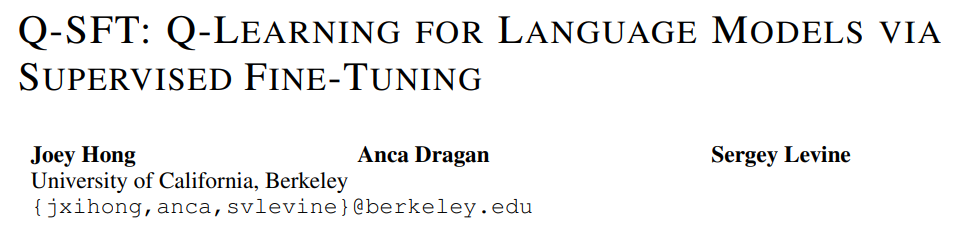
\includegraphics[width=0.8\textwidth]{img/Q-SFT head.png}
        % \caption{Q-SFT}
    \end{figure}
\end{frame}

\begin{frame}{The Core Idea: Q-Learning as SFT}
  \begin{itemize}[<+->]
    \item Reframe Q-learning as a supervised fine-tuning problem using an offline dataset $\mathcal{D} = \{(s_i, a_i, r_i)\}_{i=1}^N$.
    \item Finetune a base model to output probabilities $\hat{p}_\theta (a | s)$ that are estimates of the optimal Q-values, $Q^*(s,a)$. 
    \item (At inference time, we'll have to modify $\hat{p}_\theta$ slightly to get a good (non-greedy) policy $\pi_\theta$.)
  \end{itemize}
\end{frame}

\begin{frame}{A Note on the Dataset}
    \begin{itemize}[<+->]
        \item In text, the dataset $\mathcal{D} = \{(s_i, a_i, r_i)\}_{i=1}^N$ has actions that are tokens and states that are token sequences.
        \item E.g. $s_i$ might be the question and partial response, \texttt{"Q: If a right-angled triangle has side lengths 3 and 4, what is the length of the hypotenuse? A: We can use"}.
        \item And $a_i$ might be the next token, \texttt{"Pythagoras"}.
        \item Only the final token can have a non-zero reward, but any token can have positive values of the Q-function (\texttt{"Pythagoras"} is a good action, but \texttt{"Fermat"} is not).
        \item We can extend this to multi-turn interactions by concatenating the previous responses to the question (in which case we may get intermediate rewards).
    \end{itemize}
\end{frame}


\begin{frame}{Behavioural Cloning}
    \begin{itemize}[<+->]
        \item We can assume our offline dataset $\mathcal{D} = \{(s_i, a_i, r_i)\}_{i=1}^N$ is generated by some behaviour policy $\pi_b$ over tokens.
        \item We can train a policy $\pi_\phi$ to match the behaviour of the dataset by minimizing the cross-entropy loss:
        $$L_{\text{CE}}(\phi) = \mathbb{E}_{(s,a) \sim \mathcal{D}} \left[ \log \pi_\phi(a | s) \right]$$
        \item This is just standard SFT, and let's us approximate $\pi_\phi \approx \pi_b$ as a reference policy later.
    \end{itemize}
\end{frame}


\begin{frame}{Weighted Cross-Entropy Loss}
    \begin{itemize}[<+->]
        \item We can modify the loss function to weight different tokens/actions with weights $w(s,a)$:
        $$L_{\text{WCE}}(\theta) = \mathbb{E}_{(s,a) \sim \mathcal{D}} \left[ w(s,a) \log p_\theta(a | s)  + (1-w(a,s)) \mathbb{E}_{a' \neq a}[\log p_\theta(a' | s)] \right]$$
        \item Optimising this will give us $\hat{p}_\theta(s,a) \approx w(s,a)\pi_b(a|s)$.% (because $\mathcal{D}$ is generated by $\pi_b$).
        \item The goal is to find weights $w(s,a)$ that make $\hat{p}_\theta(s,a) \approx Q^*(s,a)$.
        \item The authors use the \textit{empirical Bellman probability operator}:
        % $$L_{\text{WCE}}(\theta) = \mathbb{E}_{(s,a) \sim \mathcal{D}} \left[ w(s,a) \log p_\theta(a | s)  + \frac{1}{\vert \mathcal{A} \vert - 1} \sum_{a' \neq a} (1-w(a,s)) \log \pi_\theta(a' | s) \right]$$
        $$w(s,a) = \hat{\mathcal{B}}^{*}\bar{p}_{\theta}(a|s) = r + \gamma\max_{a^{\prime}}\frac{\bar{p}_{\theta}(a^{\prime}|s^{\prime})}{\pi_{b}(a^{\prime}|s^{\prime})},$$
        where $r$ is the reward of moving from $s$ to $s'$ via action $a$, and $\bar{p}_{\theta}$ is a moving average of $p_{\theta}$ over training.
        \item They prove that this leads to $\hat{p}_\theta$ being a good (``conservative'') approximation of $Q^*$.
        % $$Q^*(s,a) \geq \hat{p}_\theta(s,a) \geq \pi_b(a|s)Q^*(s,a)$$
        % for all $s \in \mathcal{D}$ and $a \in \mathcal{A}$ such that $Q^*(s,a) \geq \frac{1}{\vert \mathcal{A} \vert - 1}$.
        
    \end{itemize}
  \end{frame}


\begin{frame}{Q-SFT: Policy Extraction}
    We want to extract a policy $\hat{\pi}$ from the Q-SFT model.
    \begin{itemize}[<+->]
        \item Greedy policy: $\hat{\pi}(a|s) = \mathbf{1}[a = \arg \max_a Q^*(s,a)]$.
        \item Entropy-regularised policy: $\hat{\pi}(a|s) \propto \exp(Q^*(s,a))$.
        \item KL-regularised policy (suggested by the authors) with hyperparameter $\beta > 0$: 
        $$\begin{aligned}
            \hat{\pi}(a|s) &\propto \pi_b(a|s) \exp(\beta Q^*(s,a)) \\ &\approx \pi_\phi(a|s) \exp(\beta p_\theta(a|s))
        \end{aligned}$$
        This is a well-known solution to the constrained optimisation problem:
        $$\begin{aligned}
            \arg \max_{\pi} \mathbb{E}_{s\sim P(\cdot), \; a\sim \pi(\cdot|s)}\left[Q^*(s,a)\right] \;\; s.t. \;\;
            \mathbb{E}_{s \sim P(\cdot)}\left[D_{\text{KL}}(\pi(\cdot|s) \parallel \pi_b(\cdot|s))\right] \leq \epsilon
        \end{aligned}
        $$
    \end{itemize}
\end{frame}

\begin{frame}{The Q-SFT Algorithm}
    \begin{figure}
        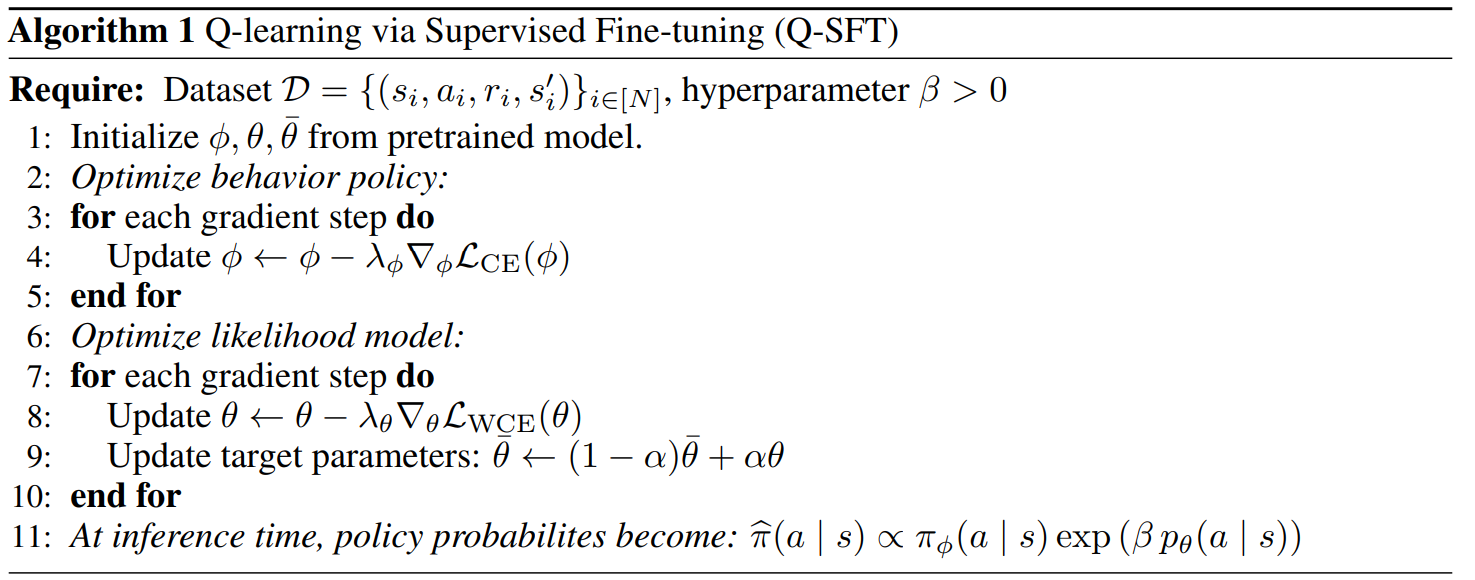
\includegraphics[width=0.8\textwidth]{img/Q-SFT algo.png}
        % \caption{Q-SFT}
    \end{figure}
\end{frame}

\begin{frame}{Experiment Settings}
    \begin{figure}
        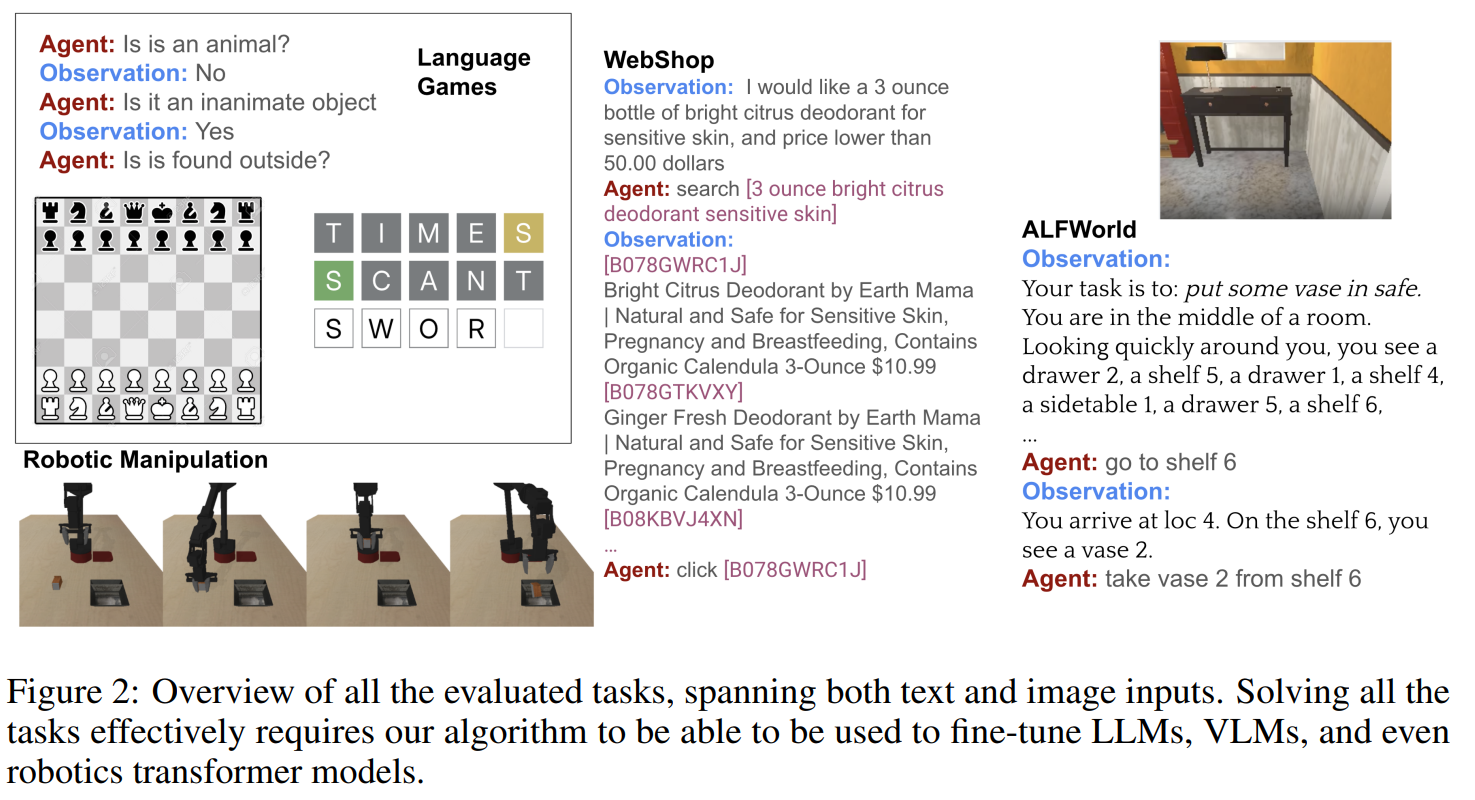
\includegraphics[width=0.8\textwidth]{img/Q-SFT tasks.png}
    \end{figure}
\end{frame}

\begin{frame}{Experimental Results}
    \begin{figure}
        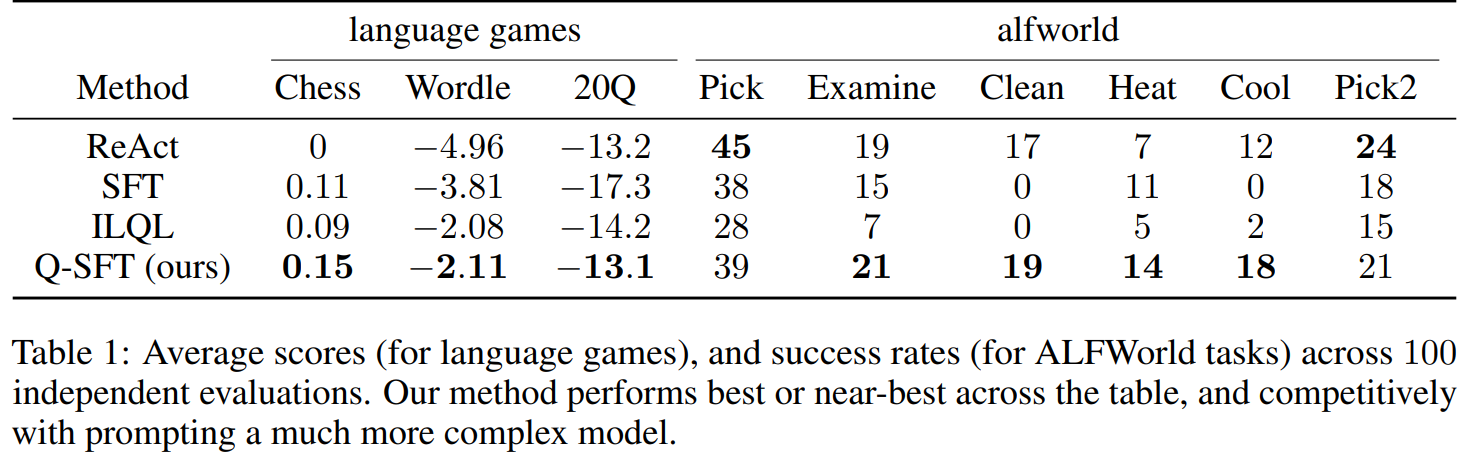
\includegraphics[width=0.8\textwidth]{img/Q-SFT eval1.png}
    \end{figure}
    \begin{itemize}
        \item ReAct: CoT/prompt-based reasoning
        \item SFT: just using $\pi_\phi$
        \item ILQL (Implicit Language Q-Learning): train an additional transformer to predict the Q-values directly.
    \end{itemize}
\end{frame}


\begin{frame}{Experimental Results}
    \begin{figure}
        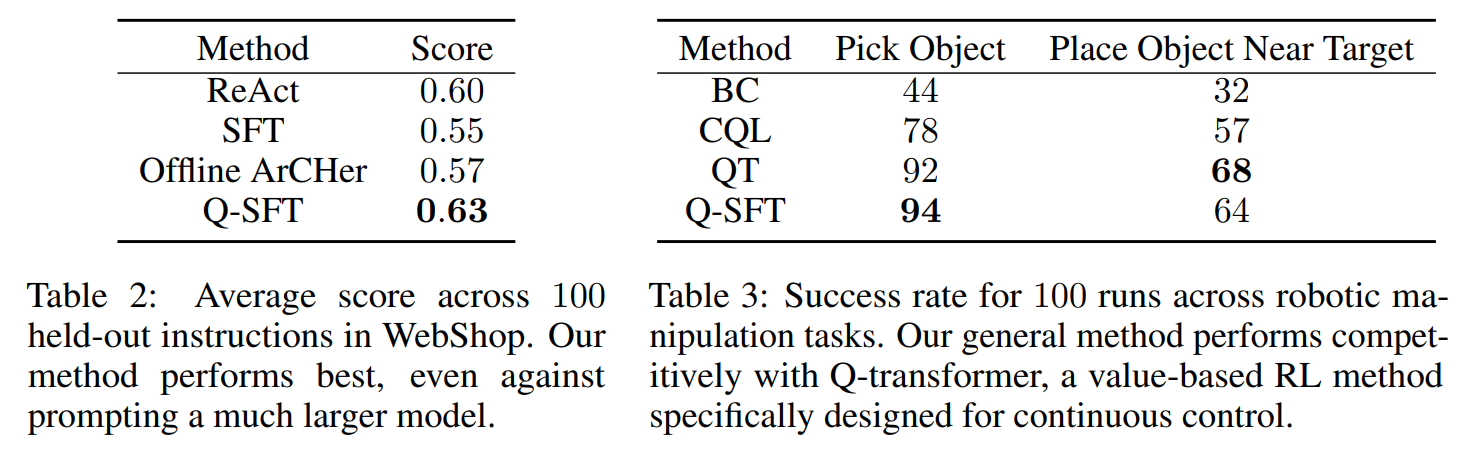
\includegraphics[width=0.8\textwidth]{img/Q-SFT eval2.png}
    \end{figure}
    \begin{itemize}
        \item ReAct: CoT/prompt-based reasoning
        \item SFT/BC (behavioural cloning): just using $\pi_\phi$
        \item Offline ArCHer: hierarchical value modelling at multi-turn-level \& token-level (seems complicated).
        \item CQL (Conservative Q-Learning) \& QT (Q-Transformer): train Q-value networks.
    \end{itemize}
\end{frame}


\begin{frame}{Experimental Results}
    \begin{figure}
        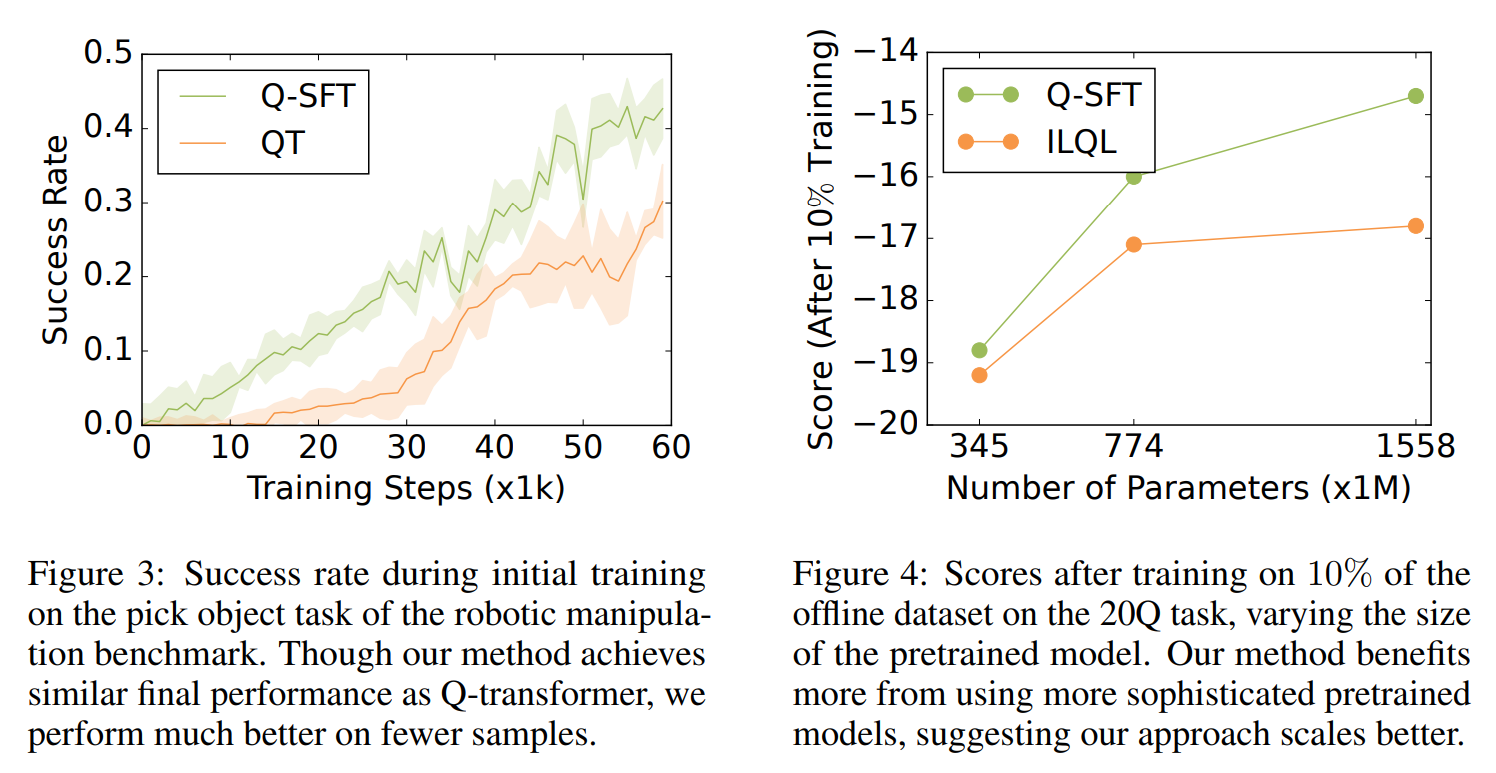
\includegraphics[width=0.7\textwidth]{img/Q-SFT eval3.png}
    \end{figure}
    \begin{itemize}
        \item (Left) Q-SFT scales better than QT with fewer samples.
        \item (Right) Q-SFT scales better than ILQL with more parameters. (``We only train on 10\% of the dataset, so that retaining prior knowledge from pretraining becomes crucial''...)
    \end{itemize}
\end{frame}
  
  \begin{frame}{Summary of Contributions}
    \begin{itemize}
      \item Reframes Q-learning as a supervised fine-tuning problem using a weighted cross-entropy loss (good for stability and simplicity).
      \item An effective way to leverage pretrained models without adding new layers or heads (this seems worthwhile).
      \item But requires training two models, $\pi_\phi$ and $\hat{p}_\theta$, plus the moving average $\bar{p}_\theta$.
      \item Some of the choices seem a bit arbitrary (e.g. the moving average to help with stability) and/or not well-motivated/explained.
      \item No comparison to online methods? 
    \end{itemize}
  \end{frame}


% % --- Part 4: Shi-Q ---
% \section{Shi-Q}

% \begin{frame}{Shi-Q}
%     \begin{figure}
%         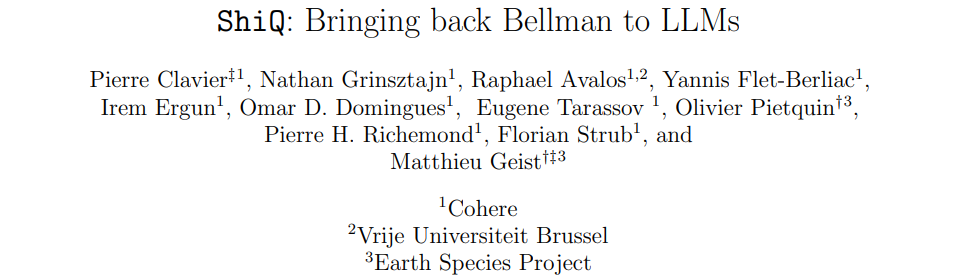
\includegraphics[width=0.8\textwidth]{img/ShiQ head.png}
%         % \caption{Shi-Q}
%     \end{figure}
% \end{frame}

% \begin{frame}{The Core Idea: Shi-Q}
%   \begin{itemize}[<+->]
%     \item ewfsgdgsd
%   \end{itemize}
% \end{frame}

% \begin{frame}{}
% %   \begin{center}
%     % \Large Any questions?
% %   \end{center}
% \end{frame}

% % % --- Part 5: Our thing ---
% \section{Our thing}

% \begin{frame}{Our thing}
%   \begin{itemize}[<+->]
%     \item Recall $Q(a|s) = $ expected future reward from action $a$ in state $s$.
%     \item If the reward is binary, $Q(a|s) = \mathbb{P}(r=1|s,a)$.
%     \item So we can think of $Q$ as a classifier that predicts the reward for a given state-action pair.
%     \item To modify the policy $P_\theta$ via $Q(a|s)$ we can use DPO-inspired approach:
%     $$P_\theta(a|s) - P_\text{ref}(a|s) = Q(a|s).$$
%     \item Training $Q$ (by updating $\theta$) as a classifier with standard supervised learning loss will give us a policy $P_\theta$ that is better than the reference policy.
%   \end{itemize}
% \end{frame}

% % --- Part 6: Results and Conclusion ---
% \section{Results and Conclusion}


% \begin{frame}{Q\&A}
%   \begin{center}
%     \Large Any questions?
%   \end{center}
% \end{frame}

\end{document}